\documentclass[conference]{IEEEtran}
\IEEEoverridecommandlockouts

\usepackage{cite}
\usepackage{amsmath,amssymb,amsfonts}
\usepackage{booktabs}
\usepackage{algorithmic}
\usepackage{graphicx}
\usepackage{textcomp}
\usepackage{xcolor}
\usepackage{caption}
\graphicspath{{../experiments/}}
\def\BibTeX{{\rm B\kern-.05em{\sc i\kern-.025em b}\kern-.08em
    T\kern-.1667em\lower.7ex\hbox{E}\kern-.125emX}}
\begin{document}

\title{Learning-Augmented MPC for Attitude Control
}

\author{\IEEEauthorblockN{Gianluca Byrnes}
}

\maketitle

\begin{abstract}
Spacecraft attitude control is a fundamentally nonlinear problem, though most
industry spacecraft systems still rely on Linear Quadratic Regulators (LQR) due to their
predictable response and computationally lightweight results. However, because LQR
control depends on a model of the system, its performance degrades when the
true spacecraft dynamics deviate from the modeled dynamics. This can be caused by multiple 
effects, such as: control input bias, external disturbances, or changes in the mass distribution.
As we enter the age of reusable spacecraft, having controllers that can adapt to 
unknown wear and tear is an attractive prospect. What kind of performance improvements
could we see if a controller was both better at handling nonlinear systems, and 
could adapt on the fly to the changing dynamics of the system?

In this project, I implement and compare three controllers for rigid-body
attitude control: a baseline LQR controller, a nominal Model Predictive
Control (MPC) controller, and a Learning-Augmented MPC (LMPC) controller.
LMPC incorporates a MLP neural network that is trained to learn
the residual dynamics function, allowing the controller to adapt to model changes.
In this analysis I have strictly used offline learning to demonstrate the 
best case scenario. Results show that nominal MPC
consistently outperforms LQR in convergence speed and overshoot reduction.
Under low to moderate model mismatch, LMPC shows the best 
performance from its model predicting ability. However, at high levels of model error,
LMPC becomes unstable due to the non-smooth residual model predictions,
and its feedback effects. 
\end{abstract}

\section{Introduction}
Attitude control is one of the most fundamental problems for spacecraft operation, nearly
every onboard system including, power generation, communication, and
navigation, depends on maintaining an precise orientation. Achieving this reliably
is challenging as spacecraft follow rigid body rotational dynamics, which are highly
nonlinear.

Despite this, the industry's gold standard remains LQR due to its predictability,
computational efficiency, and stability guarantees. Though it relies on a linearized
model of the dynamics, only useful around a small region of the linearization point.
This fact becomes more relevant as the true model deviates from the nominal model, where 
performance will degrade and the useful region becomes smaller.
To properly address the new age of reusable spacecraft, where wear and tear is expected,
controllers should be built to be robust to modeling errors.

This project explores the integration of a learned residual dynamics model 
with a MPC controller, seeking to improve both the nonlinear handling and 
the performance under model error.

\section{Spacecraft Dynamics Modeling}
In this project I have decided to use the quaternion representation for absolute orientation, 
this was done for several reasons. Firstly, quaternions do not suffer from the issue of 
gimbal lock, by providing two representations for every angle. Secondly,
they have better numerical stability for integration. Lastly, it gets rid of the
discontinuities from Euler angle representation such as going from 360 degrees to 0.

For these reasons the spacecraft is modeled as a rigid body with a state vector consisting of
a orientation quaternion \( q \in \mathbb{R}^4 \) and an angular velocity vector
\( \omega \in \mathbb{R}^3 \).
\begin{equation}
x = \begin{bmatrix} q \\ \omega \end{bmatrix} \in \mathbb{R}^7
\end{equation}

The continuous-time dynamics for the spacecraft are given by quaternion rigid body mechanics:
\begin{align}
\dot{q} &= \frac{1}{2}\Omega(\omega) q, \\
\dot{\omega} &= I^{-1}(\tau - \omega \times (I\omega)),
\end{align}
where \( I \) is the inertia matrix and \( \tau \) is the applied control
torque.

Although quaternion representation is optimal for representing absolute rotation,
it presents issues when linearization is involved. For a quaternion to represent a
valid rotation it must be of unit length. This is not viable when you linearize around a quaternion.

To circumvent this issue, the controllers implement error coordinates for orientation
as Euler angles instead of quaternions. This converts the state space to a 6D representation
inside the controller. The Euler error angle vector can be approximated as the following: 
\begin{align}
q_{\text{err}} &= q_{\text{goal}}^{-1} \otimes q_{\text{curr}} \\
\implies q_{\text{err}} &= \begin{bmatrix} \cos\left(\frac{\|\theta_{\text{err}}\|}{2}\right) \\ \frac{\theta_{\text{err}}}{\|\theta_{\text{err}}\|}\sin\left(\frac{\|\theta_{\text{err}}\|}{2}\right) \end{bmatrix} \\
\implies q_{\text{err}} &\approx \begin{bmatrix} 1 \\ \frac{1}{2}\theta_{\text{err}} \end{bmatrix}
\end{align}

The error state vector is then given by:
\begin{equation}
x_{\text{err}} = \begin{bmatrix} \theta_{\text{err}} \\ \omega_{\text{err}} \end{bmatrix} \in \mathbb{R}^6
\end{equation}
This hybrid design allows for globally accurate orientation modeling
and allows linearization.



\section{Controllers}

\subsection{Linear Quadratic Regulator}
The LQR controller is implemented as a time invariant, discrete time controller.
It uses linearized discrete time dynamics:
\begin{equation}
x_{k+1} \approx A_d x_k + B_d u_k,
\end{equation}

computed via finite differencing around the goal state. The optimal control gain \(K\)
is found using the discrete time Riccati equation, which is used to yield the optimal
control law: 

\begin{equation}
u = -Kx_{\text{err}}.
\end{equation}

The control torques are then clipped to the actuator limits.
This controller serves as the baseline for comparison.


\subsection{Nominal Model Predictive Control}
The nominal MPC controller is implemented as a linear multiple shooting MPC 
controller. This flavor of MPC provides good computational efficiency, by keeping constrains linear,
while also being well suited for handling nonlinear problems. 
It is formulated as a finite-horizon quadratic program over a
prediction horizon \(N\) (set to 30 points in all experiments):
\begin{equation}
\min_{x_{0:N}, u_{0:N-1}} 
\sum_{k=0}^{N-1} (x_k^\top Q x_k + u_k^\top R u_k)
+ x_N^\top Q_f x_N,
\end{equation}
subject to
\begin{align}
x_{k+1} &= A_k x_k + B_k u_k, \\
u_{\min} &\le u_k \le u_{\max}.
\end{align}
Like in the LQR case, the linearized dynamics are computed using finite differencing.

The controller was built using Drake's \texttt{MathematicalProgram}
where I defined decision variables, quadratic costs, and constraints on the 
dynamics and control torques. The controller also implements warm start 
functionality where previously computed trajectories will be used as a starting 
initial guess to the decision variables. In the case where it is the first run, 
the initial guess is set to the linearly interpolated trajectory from current to goal
state, with zero control torque. 

The main advantage this controller over traditional LQR is its ability to 
plan a trajectory from current to goal state, while linearizing around multiple 
points in the process. The net outcome of this is that the controller is well 
informed about the dynamics across the whole trajectory, assuming the horizon
is large enough, not just at the goal state.
This allows the controller to recover from large disturbances since it can plan
a path back to the goal, instead of just "steering" linearly toward it.
This plan is iterated on each time the controller runs. 

The control torque for this controller is given as the first element of the optimized 
control trajectory.
\begin{equation}
u = u_0
\end{equation}

\subsection{Learning-Augmented Model Predictive Control}
The Learning-Augmented MPC (LMPC) controller extends the nominal MPC 
by incorporating a learned model of the residual dynamics. This addition seeks
to create a more robust controller to effects of model error.

The true rigid body dynamics can be separated into a nominal component  
and a residual component:
\begin{equation}
f_{\text{true}}(x,u) = f_{\text{nominal}}(x,u) + r(x,u),
\end{equation}
where \( r(x,u) \) captures the unmodeled effects. In this project,
the residual function is approximated by training a multilayer perceptron (MLP), 
on data generated from closed-loop simulations with intentionally injected model errors. 
The MLP was made with 17k parameters, containing 3 hidden layers [64, 64, 32], and using 
the RELU activation function.
Each entry in the dataset contains the 
current state, current control input, the next state predicted using the nominal  
model, and the true next state from the simulator. The MLP learns to predict 
the residual of the discrete time dynamics
\begin{equation}
r_\theta(x_k,u_k) \approx f_{\text{true}}(x_k,u_k) - f_{\text{nominal}}(x_k,u_k),
\end{equation}
using mean squared prediction error as the loss.

Once trained, the model is used to create the dynamics constraints 
for the LMPC controller by linearizing the full dynamics around each point 
of the guess trajectory. Similar to nominal MPC the horizon was set to 30 points.

\begin{equation}
x_{k+1} = f_{\text{nominal}}(x_k, u_k) + r_\theta(x_k, u_k).
\end{equation}
\begin{equation}
A_k = \frac{\partial f_{\text{hybrid}}}{\partial x}\bigg|_{(x_k,u_k)}, \qquad 
B_k = \frac{\partial f_{\text{hybrid}}}{\partial u}\bigg|_{(x_k,u_k)},
\end{equation}
Like before, this is computed using finite differencing.

This formulation of the LMPC controller represents the best case scenario.
All the data to train the model is collected ahead of time, and it is on 
trained offline, with no limits on either.
This is in comparison to the more useful online approach that has limits on 
training data and training time. The results for this offline 
variant will give an upper bound of the expected performance of an online approach.

\section{Results}

\subsection{Simulation Setup}
All simulations were conducted with a timestep \( \Delta t = 0.5 \) seconds over 700 steps
, using RK4 integration for numerical accuracy. The control inputs were
constrained to a maximum torque of \( \pm 0.10 \) N\( \cdot \)m on
each axis.

To test the controller's robustness to model uncertainty,
a variety of different "real" inertia matrices were used that deviated
from the nominal inertia matrix \( I_{\text{nominal}} \). The model
error was calculated by the percentage difference in the Frobenius
norm between the true inertia matrix \( I_{\text{true}} \) and
\( I_{\text{nominal}} \), calculated as
\( \frac{\|I_{\text{true}} - I_{\text{nominal}}\|_F}{\|I_{\text{nominal}}\|_F} \times 100\% \).
I quantified the following ranges:
\begin{itemize}
    \item \textbf{Low Model Error:} A true inertia matrix with a $<$5.00\%
    difference from \( I_{\text{nominal}} \).
    \item \textbf{Moderate Model Error:} True inertia matrices with 5.00\%
    to 15.00\% differences from \( I_{\text{nominal}} \).
    \item \textbf{High Model Error:} A true inertia matrix with a $>$15.00\%
    difference from \( I_{\text{nominal}} \).
\end{itemize}
The nominal inertia matrix used for controller design was:
\[
I_{\text{nominal}} = \begin{pmatrix}
90.0 & -5.0 & 3.0 \\
-5.0 & 110.0 & -4.0 \\
3.0 & -4.0 & 100.0
\end{pmatrix} \text{ kg}\cdot\text{m}^2
\]

In addition to model uncertainty, these disturbances were included:
\begin{itemize}
    \item \textbf{Bias Torque:} A constant torque of
    \( [0.05, -0.045, 0.03] \) N\( \cdot \)m.
    \item \textbf{Gaussian Noise:} Random Gaussian noise with a standard
    deviation of \( 0.003 \) N\( \cdot \)m.
    \item \textbf{Sinusoidal Disturbance:} A sinusoidal torque with an
    amplitude of \( 0.04 \) N\( \cdot \)m and a frequency of \( 0.05 \) Hz.
\end{itemize}

\subsection{Computational Performance}

\begin{table}[htbp]
    \centering
    \caption{Controller Computational Performance}
    \label{tab:computational_performance}
    \begin{tabular}{lc}
        \large
        \toprule
        \textbf{Controller} & \textbf{Performance} \\
        \midrule
        LQR & $\sim$7000 iterations/s \\
        Nominal MPC & $\sim$20 iterations/s \\
        LMPC & $\sim$1.6 iterations/s \\
        \bottomrule
    \end{tabular}
\end{table}

\subsection{LQR vs. MPC}
Across all tests, the nominal MPC controller outperformed LQR in
terms time to convergence, overshoot, and robustness to disturbances. The nominal
MPC's ability to plan its trajectory into the future significantly helps here.

\subsection{Learning-Augmented MPC Performance}
Under low to moderate model error, LMPC improved tracking performance by
accounting for the errors in the dynamics model. LMPC had fastest convergence, 
and lowest overshoot.

However, at high model error, LMPC becomes unstable. The learned
residual model seems to be non-smooth and this leads to wild changes in control 
resulting in divergence. Surprisingly the nominal MPC and LQR controllers remain stable.


\subsection{Control Input Characteristics}
The Control inputs from LMPC show increasingly wild control inputs, proportional
the level of model error, and thus the influence of the residual model. 
This observed behavior is most likely explained by the fact that the residual model 
is non-smooth and noisy. Numerical derivatives inherently amplify noise, and using
finite differencing to compute the linearized dynamics makes the noise worse and 
this propagates to the control inputs.


\begin{figure*}[htbp]
    \centering
    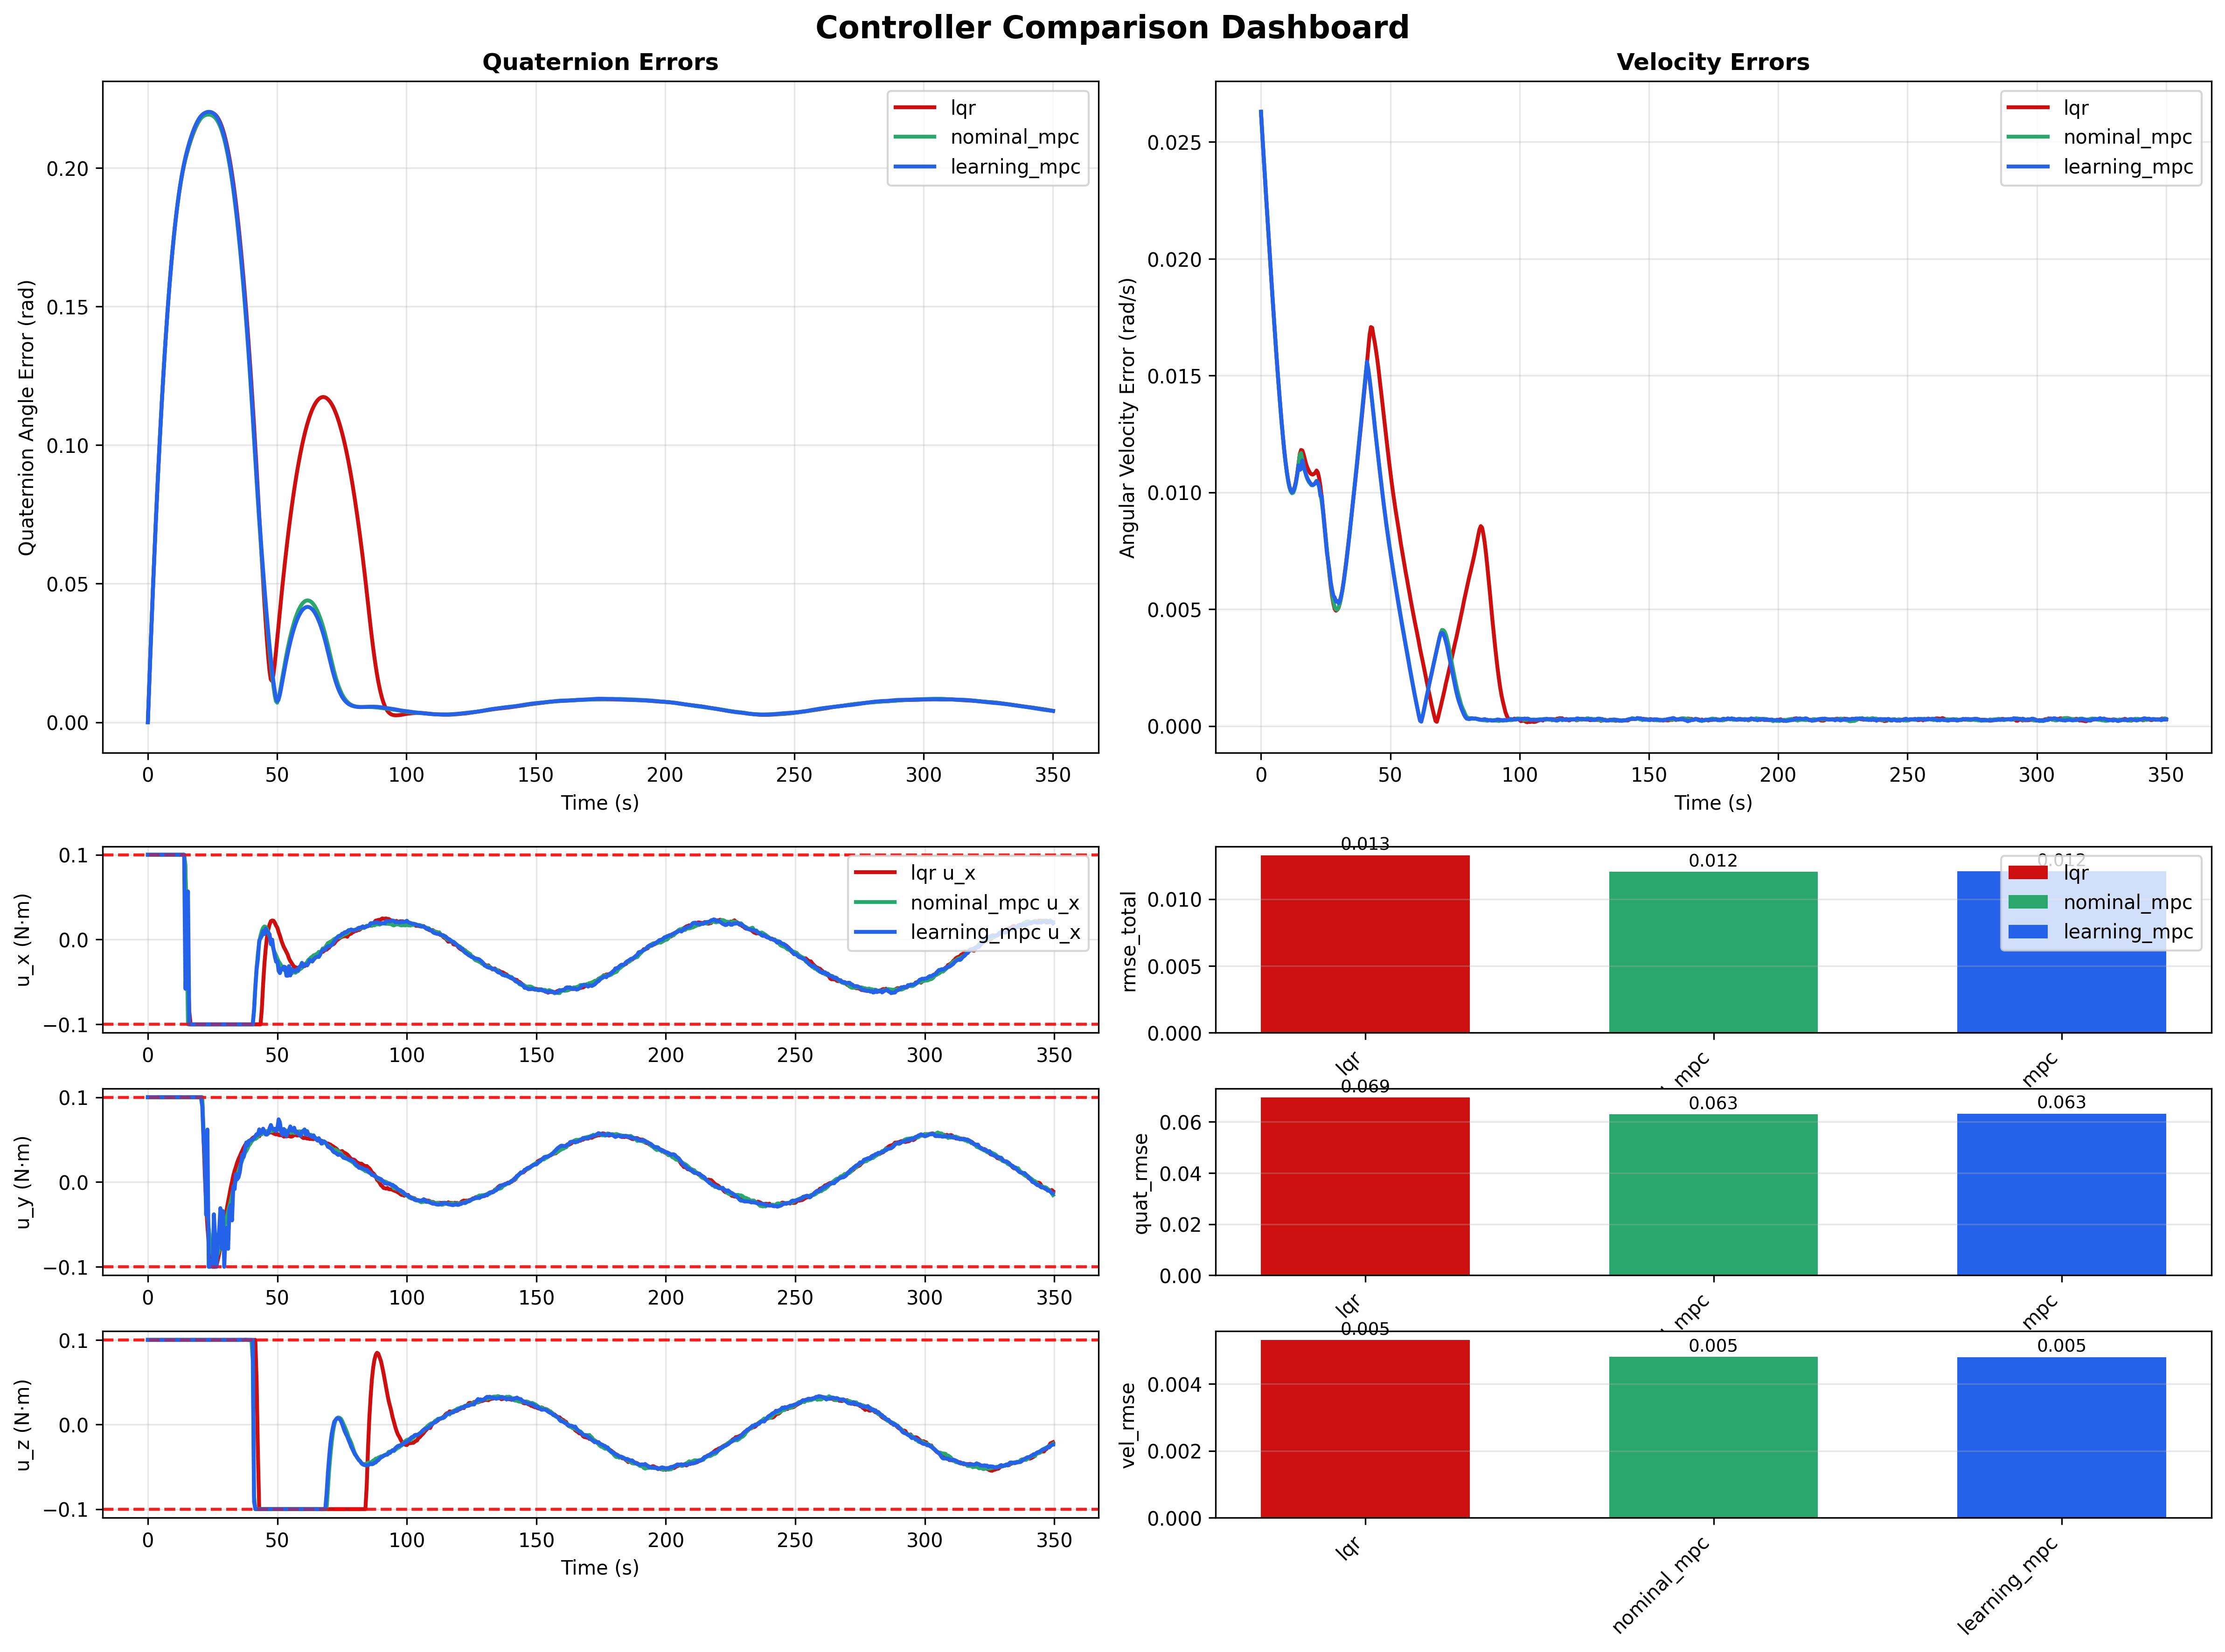
\includegraphics[width=\textwidth]{../experiments/combined_controller_comparison_5.png}
    \caption{\large Controller performance comparison with \textbf{2\% model error}. This figure illustrates the tracking performance, angular velocity, and control inputs for LQR, nominal MPC, and learning-augmented MPC under low model error conditions.}
    \label{fig:comparison_5_percent}
\end{figure*}

\begin{figure*}[htbp]
    \centering
    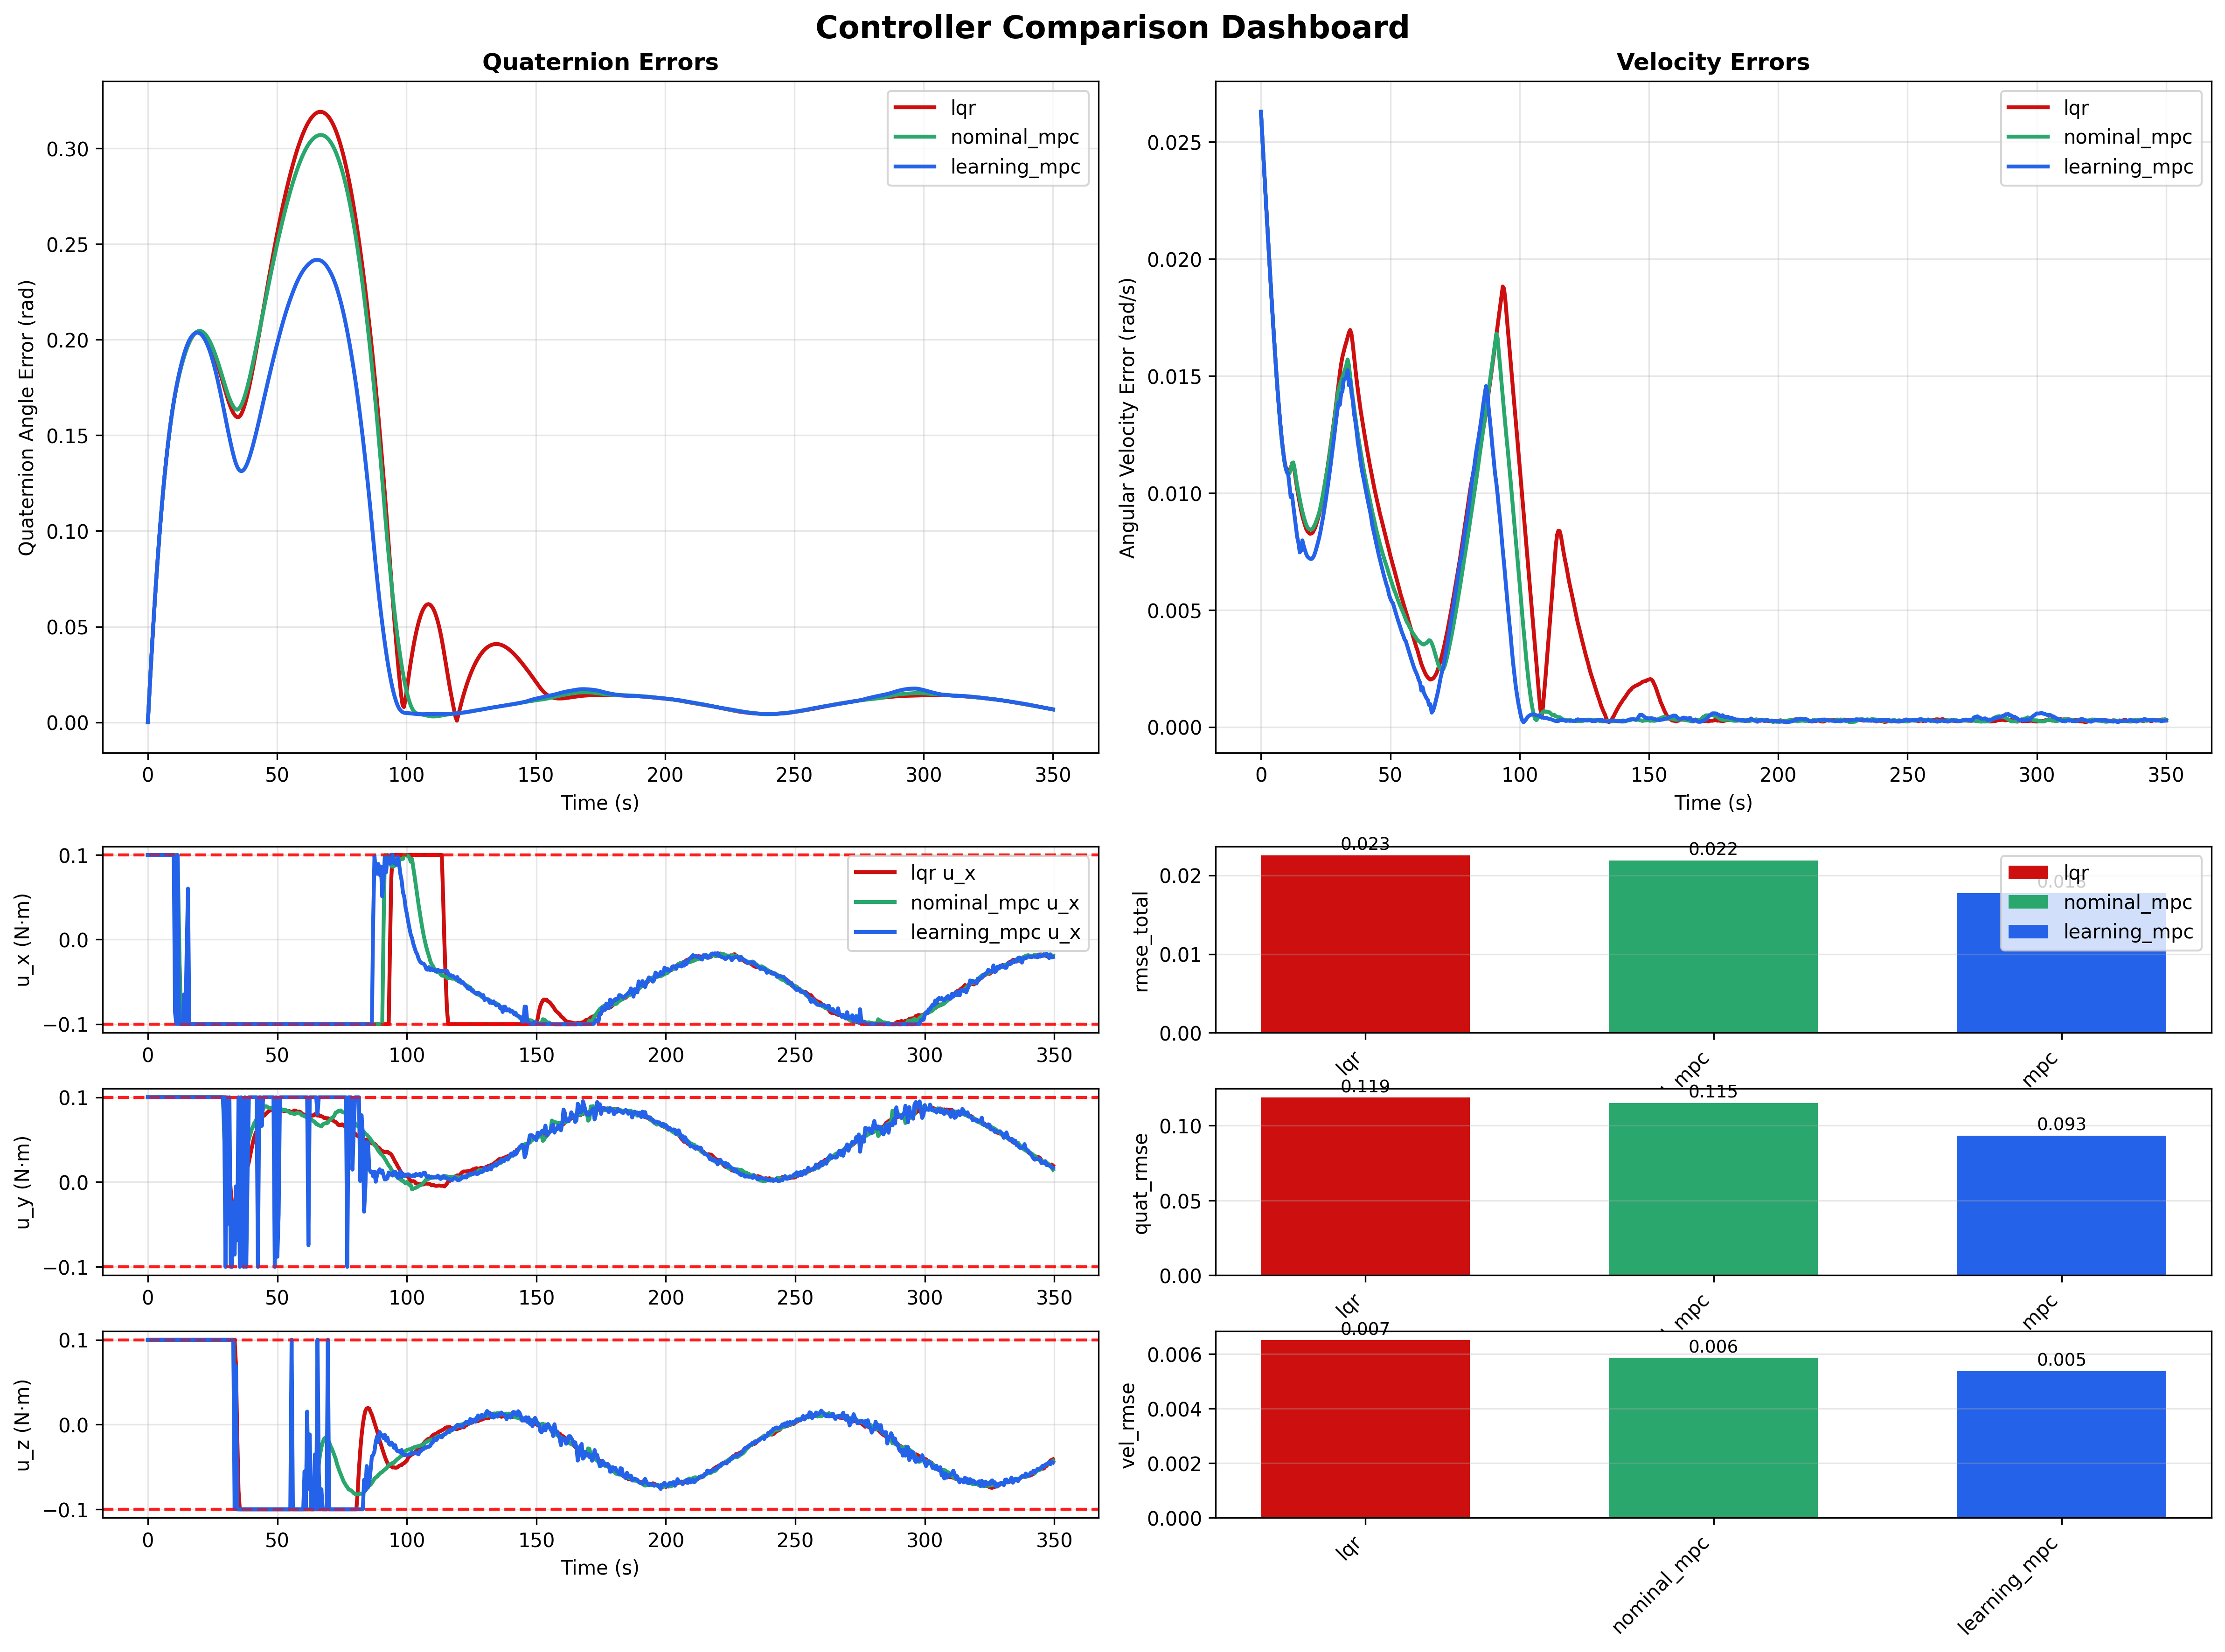
\includegraphics[width=\textwidth]{../experiments/combined_controller_comparison_15.png}
    \caption{\large Controller performance comparison with \textbf{6\% model error}. This figure illustrates the tracking performance, angular velocity, and control inputs for LQR, nominal MPC, and learning-augmented MPC under moderate model error conditions.}
    \label{fig:comparison_15_percent}
\end{figure*}

\begin{figure*}[htbp]
    \centering
    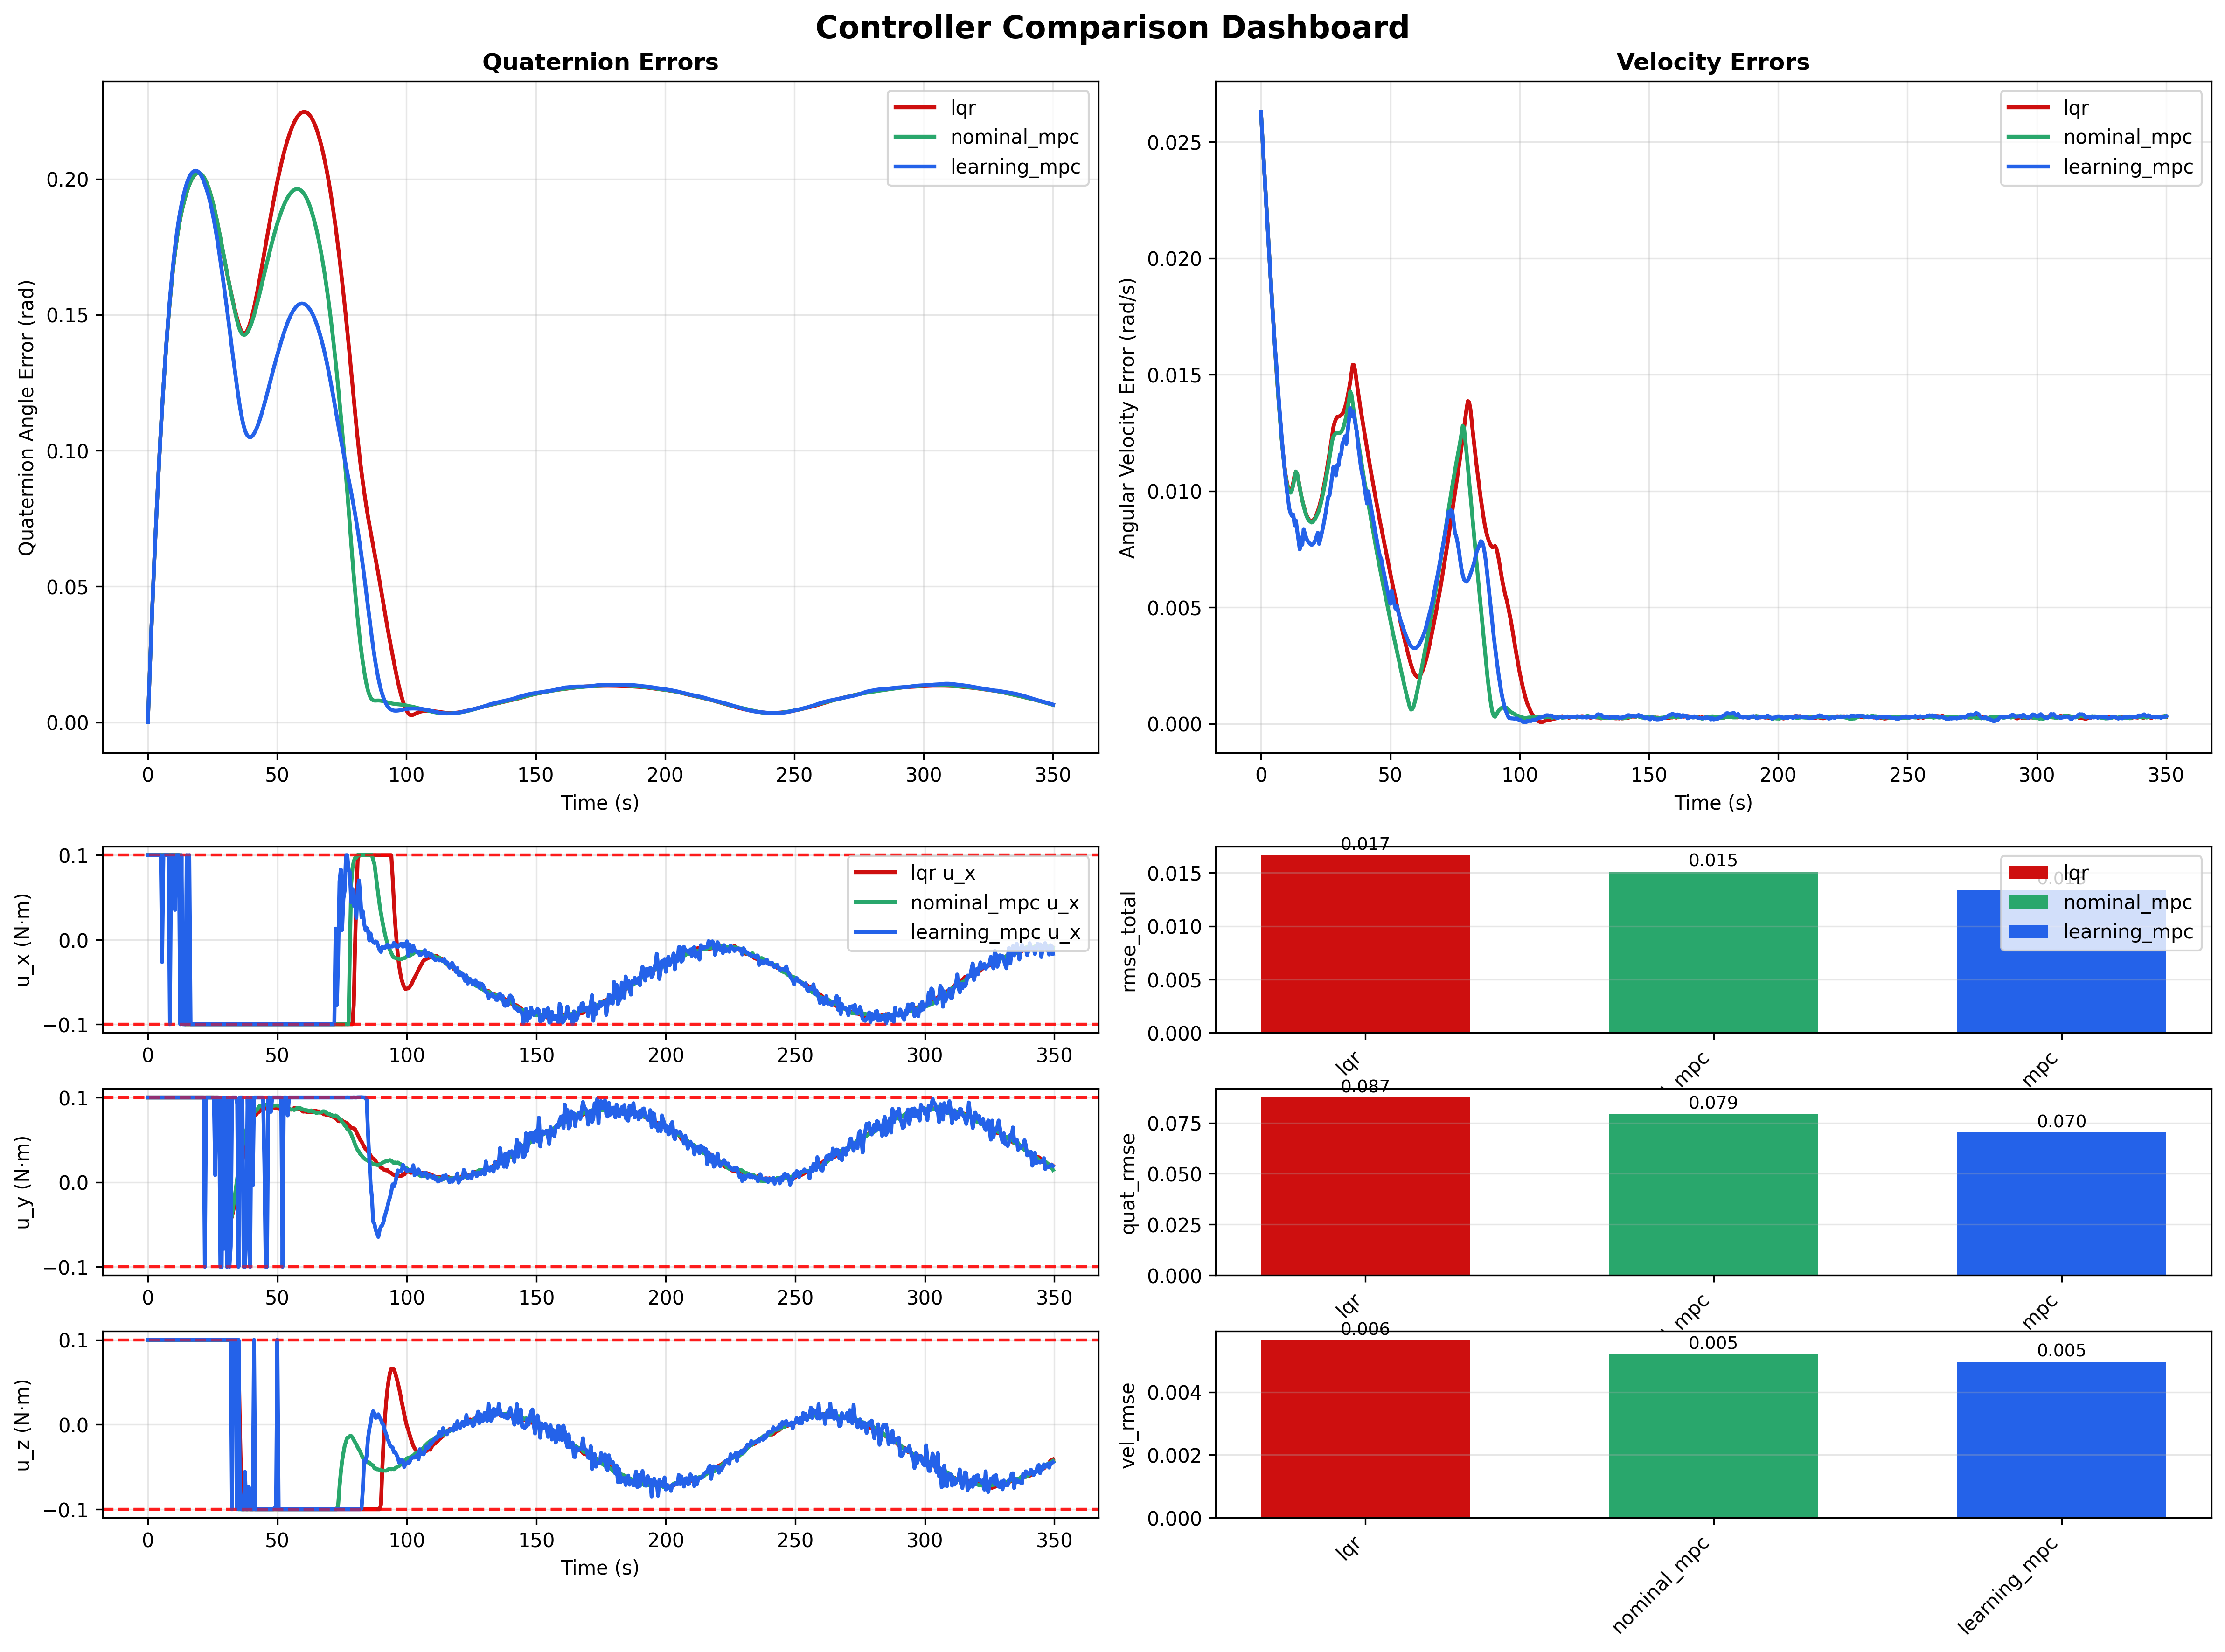
\includegraphics[width=\textwidth]{../experiments/combined_controller_comparison_25.png}
    \caption{\large Controller performance comparison with \textbf{10\% model error}. This figure illustrates the tracking performance, angular velocity, and control inputs for LQR, nominal MPC, and learning-augmented MPC under moderate model error conditions.}
    \label{fig:comparison_25_percent}
\end{figure*}

\begin{figure*}[htbp]
    \centering
    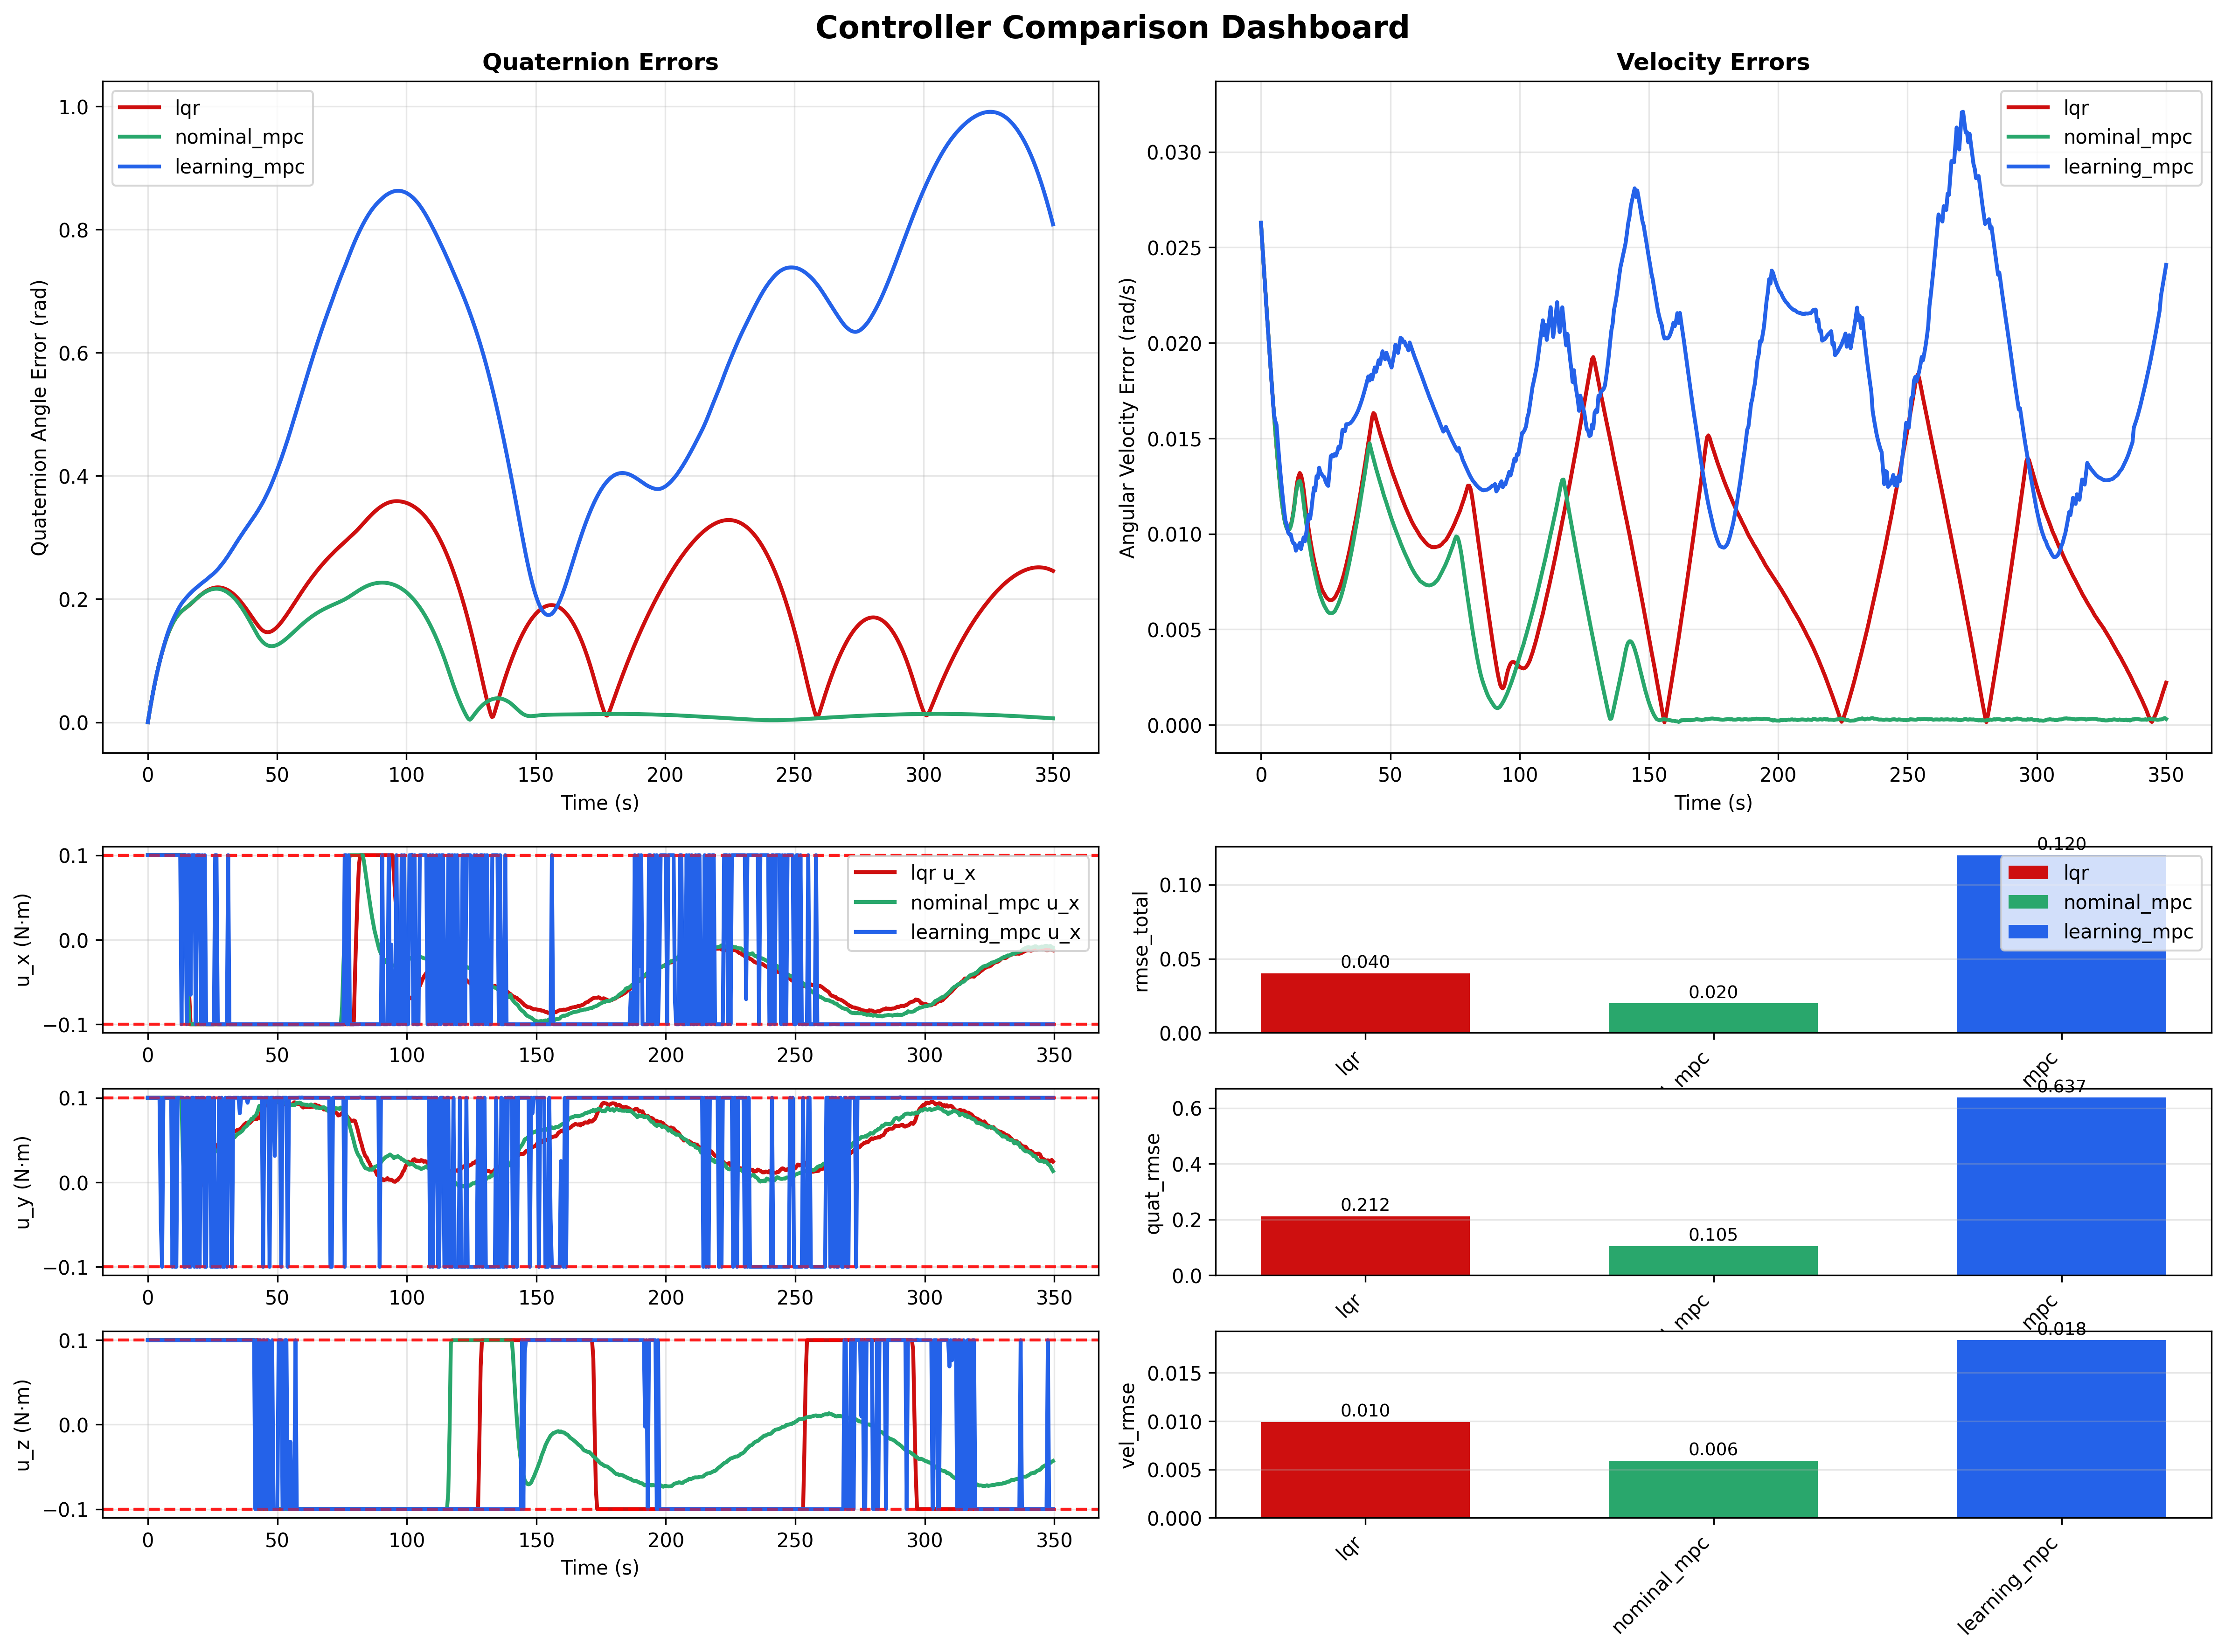
\includegraphics[width=\textwidth]{../experiments/combined_controller_comparison_full.png}
    \caption{\large Controller performance comparison with \textbf{20\% model error}. This figure demonstrates the controller performance under very high model error, highlighting the limitations of LMPC in such extreme conditions.}
    \label{fig:comparison_full_error}
\end{figure*}

\begin{figure*}[htbp]
    \centering
    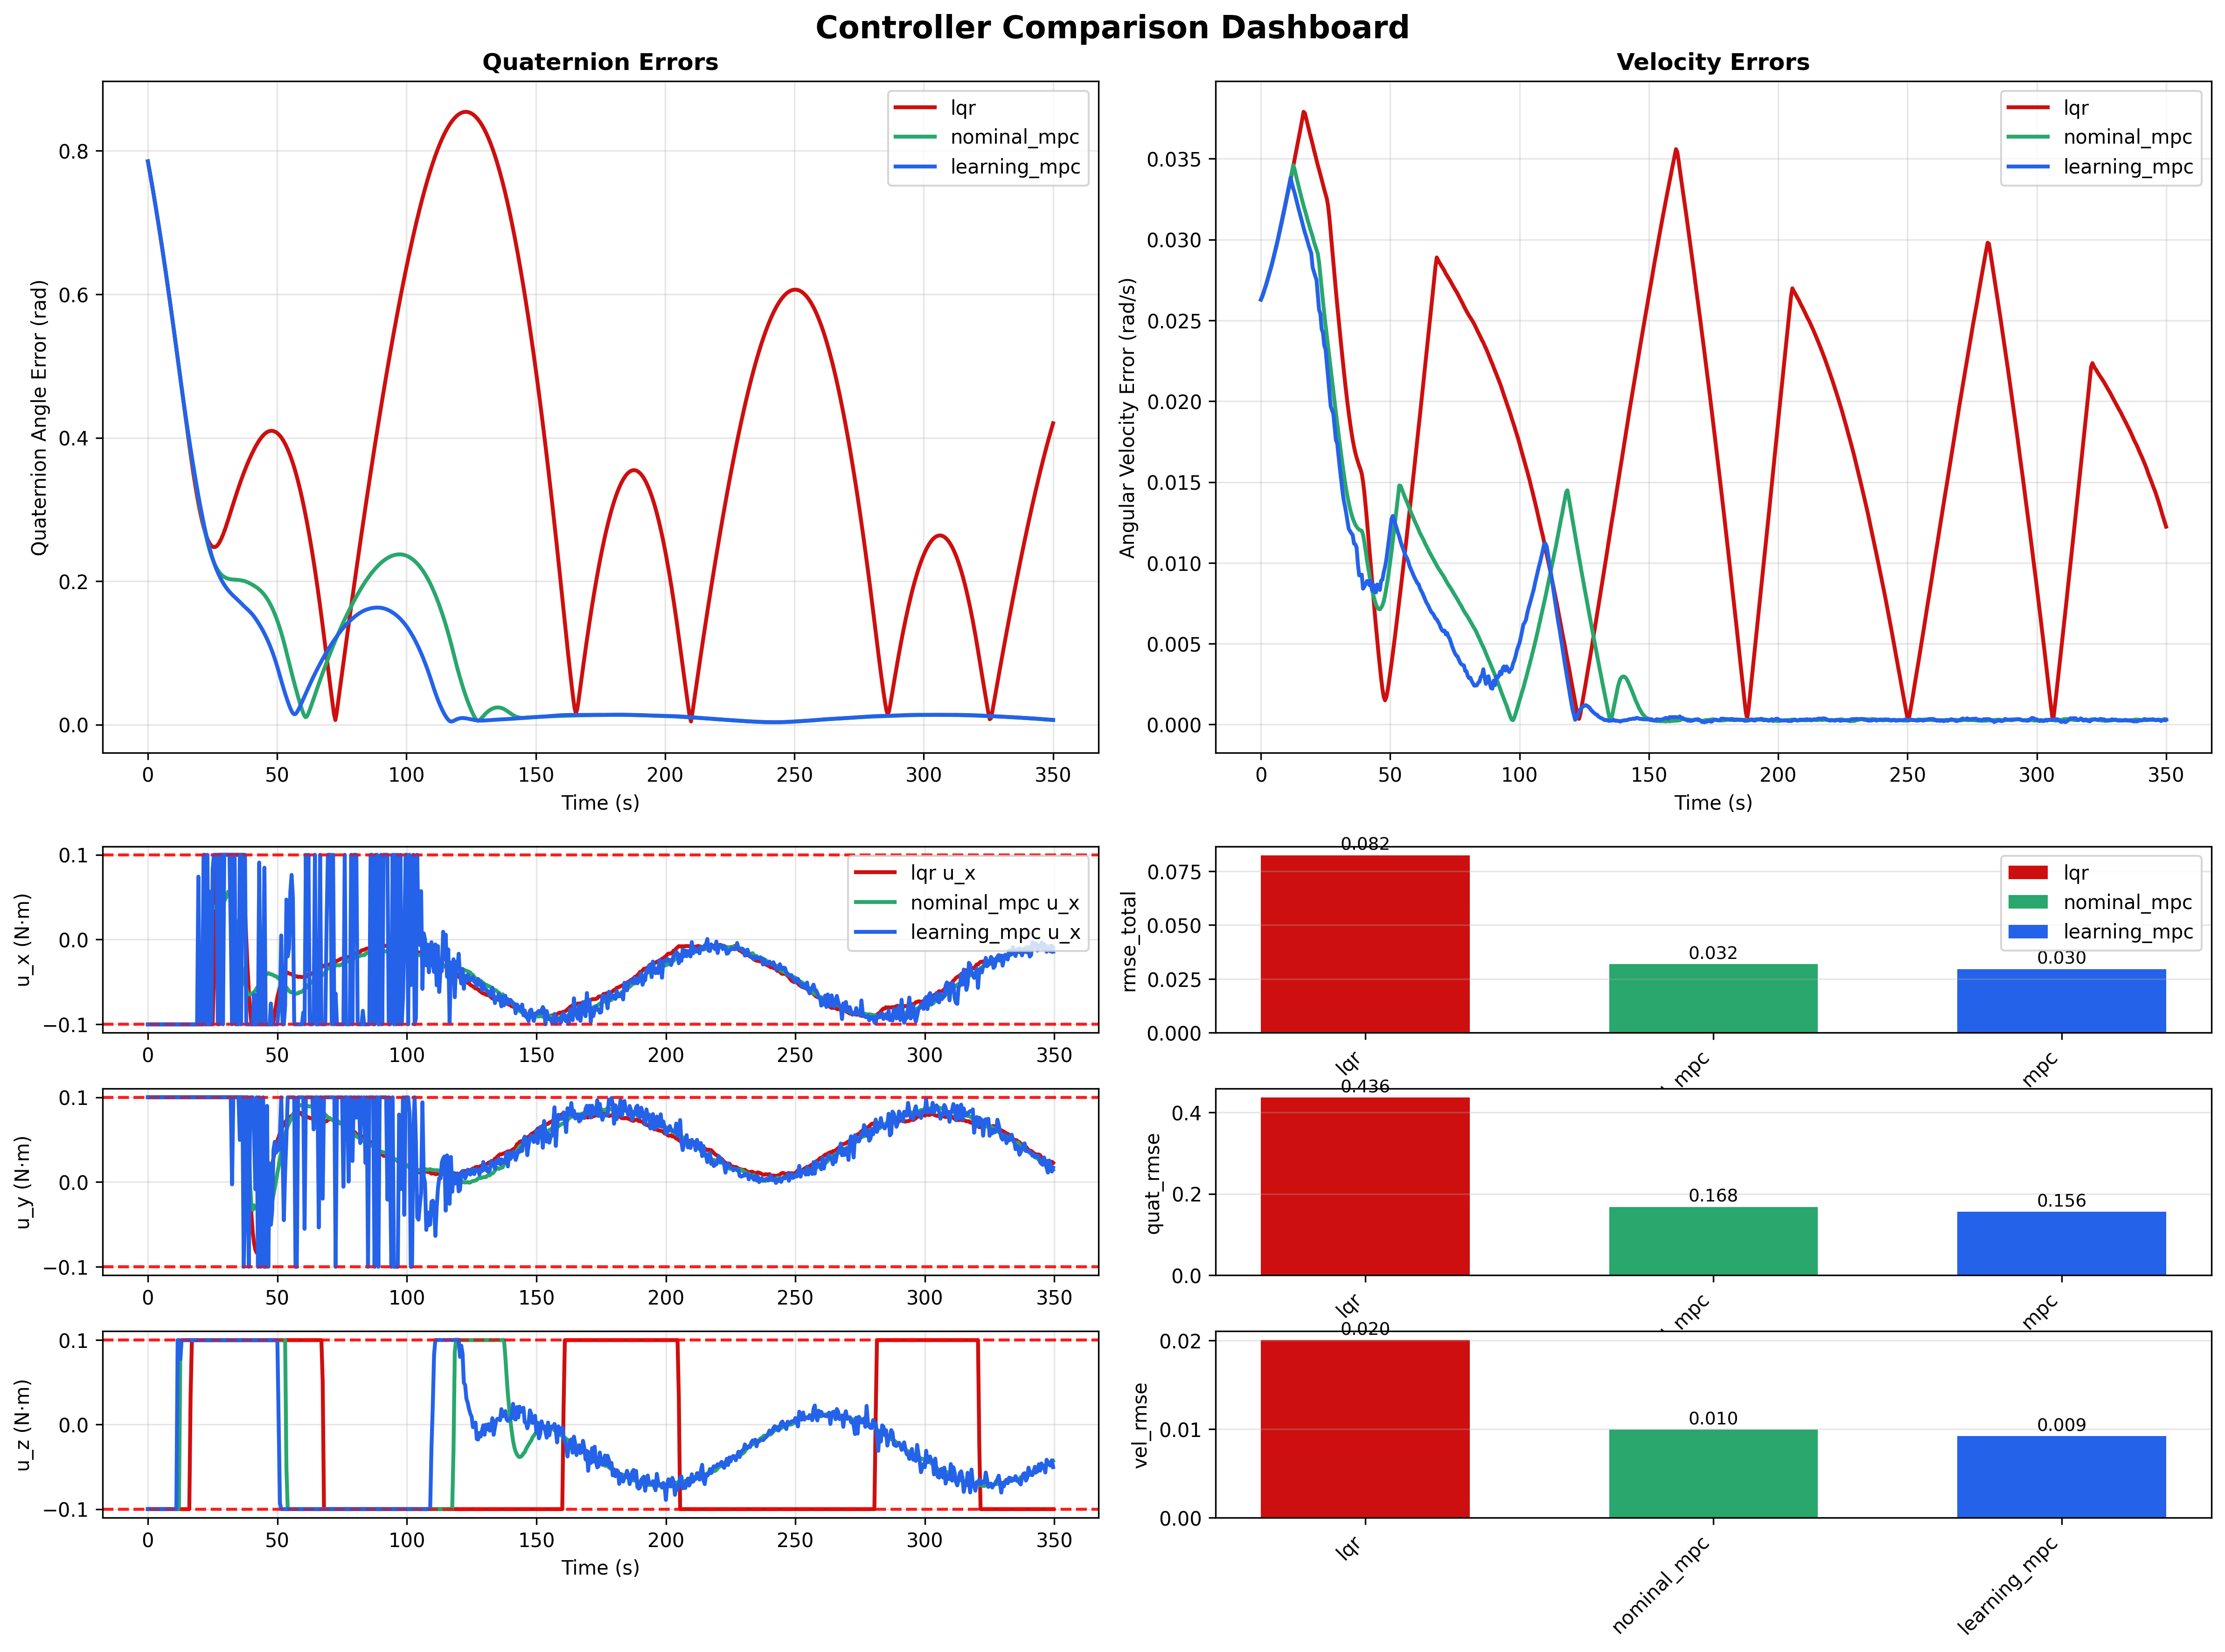
\includegraphics[width=\textwidth]{../experiments/combined_controller_comparison_25_45degree.png}
    \caption{\large Controller performance comparison with \textbf{10\% model error} and 45-degree initial orientation error. This figure shows the controller behavior under moderate model error and a significant initial state deviation.}
    \label{fig:comparison_25_percent_45deg}
\end{figure*}


\section{Discussion}

\subsection{What Worked}
\begin{itemize}
    \item The nominal MPC controller outperformed LQR in every metric other than 
computation speed.
    \item The LMPC showed promise and outperformed the other controllers
in low to moderate model error cases, where realistic scenarios would lie.
    \item The hybrid approach to representing orientation with quaternions and Euler angles
was successful.
\end{itemize}


\subsection{What Did Not Work}
\begin{itemize}
    \item LMPC preformed the worst at large model error due to the effects of the non-smoothness
and output noise of the learned residual model. Contributing factors to this are most likely the
fact I used RELU as the activation function instead of tanh, and did not have a complex enough model
architecture to effectively model the nonlinearity.
    \item The finite differencing method traded ease of implementation for computation speed, 
though this resulted in large noise in the LMPC and significantly reduced performance 
of the controller. To compute one linearized set of matrices it had to run through the 
residual model for each parameter.
\end{itemize}


\subsection{Future Work}


Future directions include:
\begin{itemize}
    \item Look into physics informed ML approaches for improving model noise and predictions.
    \item Look into improved the methods for computing the jacobian from a neural network.
    \item Explore feasibility of a online learning setup.
\end{itemize}

\end{document}
